\subsection{Github}
All code used for this project can be found at \\ \url{https://github.com/mgoretti/HEC-microeconometrics}

\subsection{IV Probit settings}
Due to the complexity of the model and number of observations, the iterating algorithm computing the maximum likelihood was having trouble converging (and taking way too much time to do so). I identified the problem in the criteria for the convergency of the method. It was using an absolute difference instead of a relative one (and a very high number of max iterations). In a normal setup this problem can be settled by changing the convergence criterium to be a relative change in maximum likelihood between steps of less than 0.01\% but stata doesn't accept so I had to settle for an ad-hoc criterium of having a norm the gradient of less than $10^{-3}$ which has the problem of not being scaled relatively to the maximum likelihood.

\subsection{Figures}
\begin{figure}[H]
\makebox[\textwidth][c]{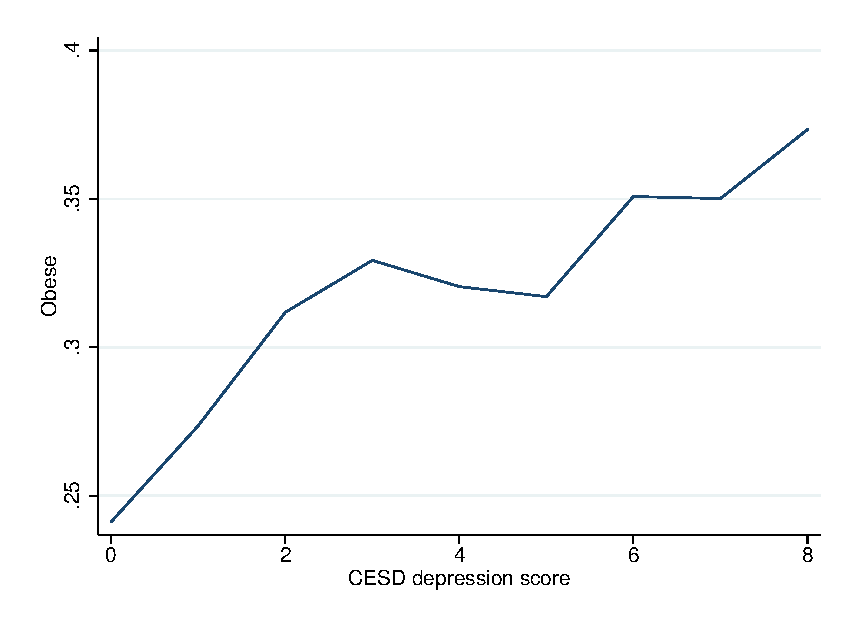
\includegraphics[width=0.6\paperwidth]{../proj/fig/obesity.eps}}
\caption{Percentage of obese persons as a function of their depression }
\label{fig:obesity}
\end{figure}

\begin{figure}[H]
\makebox[\textwidth][c]{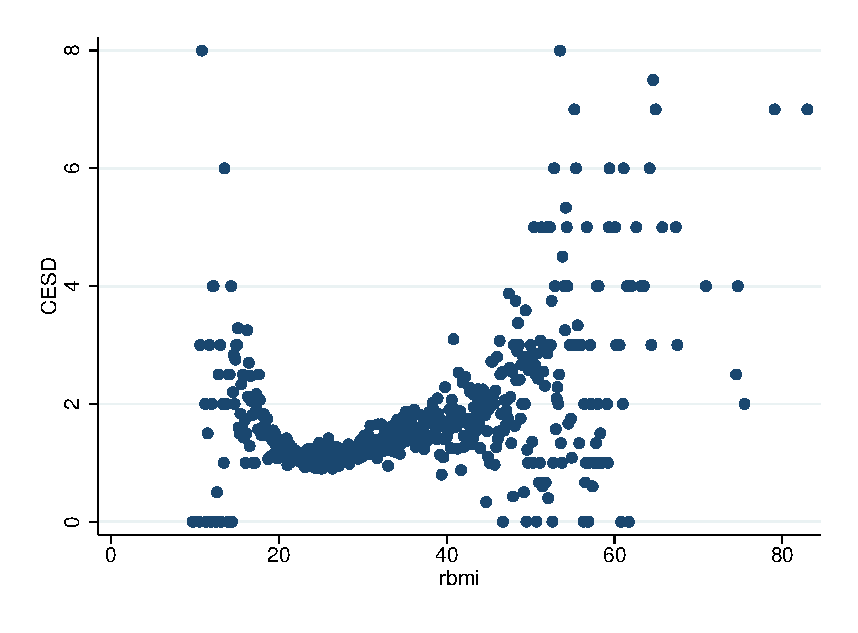
\includegraphics[width=0.6\paperwidth]{../proj/fig/cesd.eps}}
\caption{Mean depression as a function of the BMI}
\label{fig:cesd}
\end{figure}


\begin{figure}[H]
\makebox[\textwidth][c]{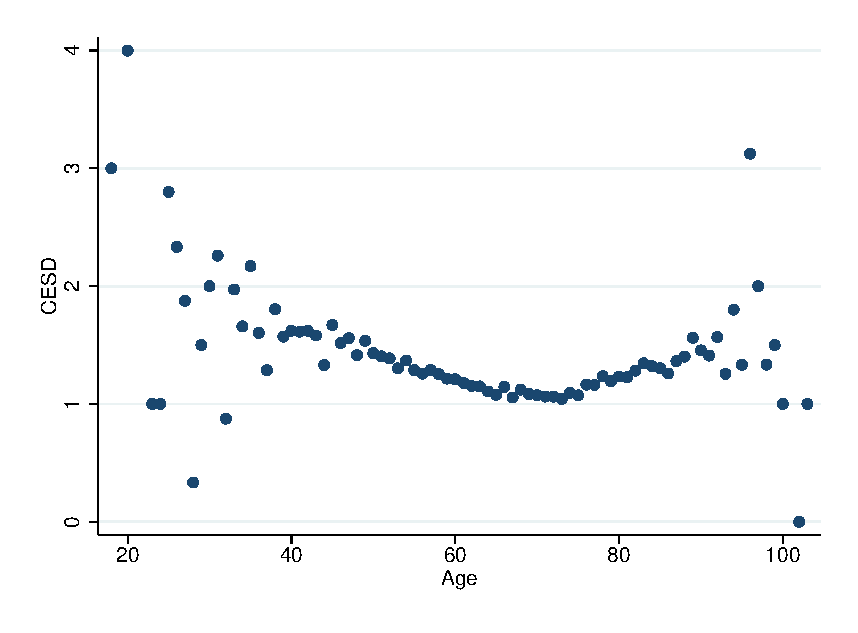
\includegraphics[width=0.6\paperwidth]{../proj/fig/agecesd.eps}}
\caption{Mean depression score as a function of the age}
\label{fig:agecesd}
\end{figure}



\begin{figure}[H]
\makebox[\textwidth][c]{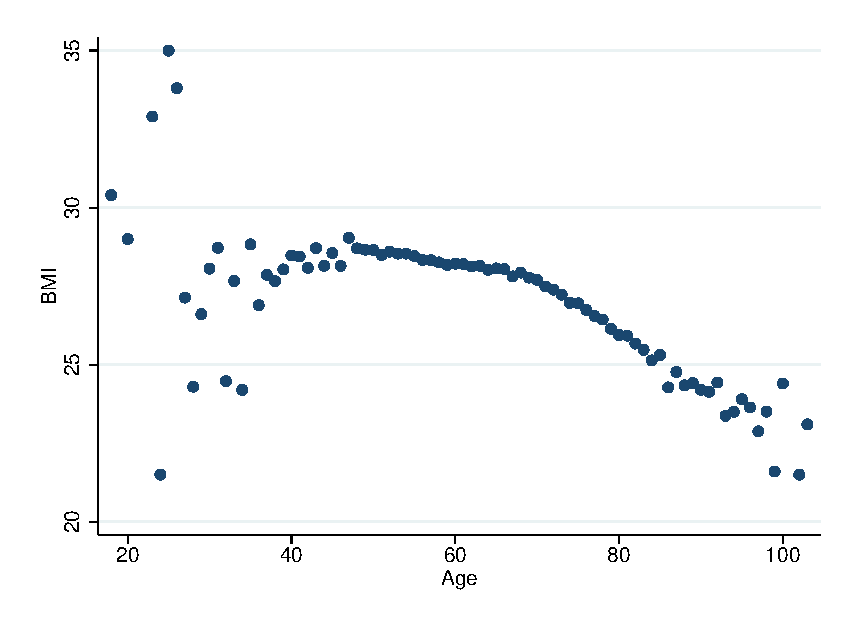
\includegraphics[width=0.6\paperwidth]{../proj/fig/agebmi.eps}}
\caption{Mean bmi as a function of the age}
\label{fig:agebmi}
\end{figure}

\begin{figure}[H]
\makebox[\textwidth][c]{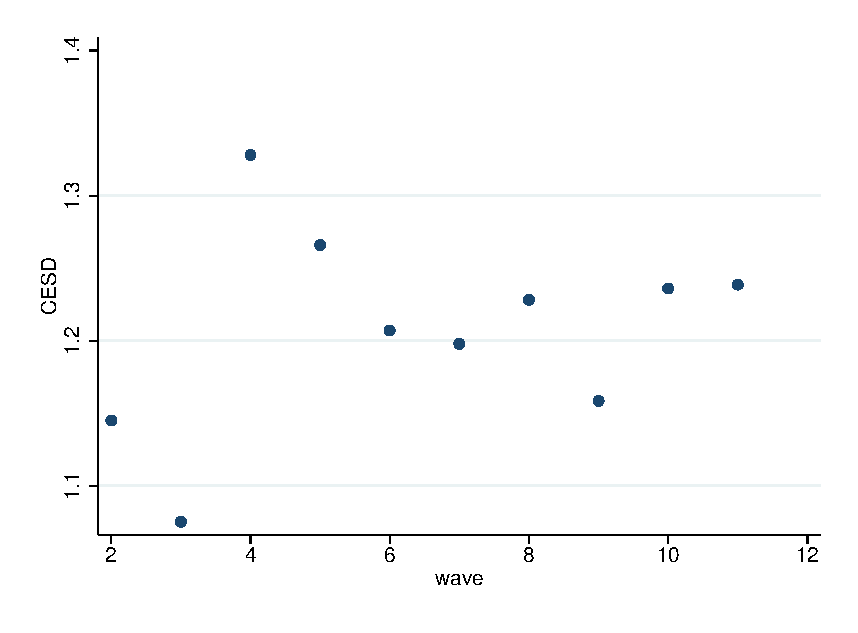
\includegraphics[width=0.6\paperwidth]{../proj/fig/wavecesd.eps}}
\caption{Mean depression score as a function of the wave}
\label{fig:wavecesd}
\end{figure}

\begin{figure}[H]
\makebox[\textwidth][c]{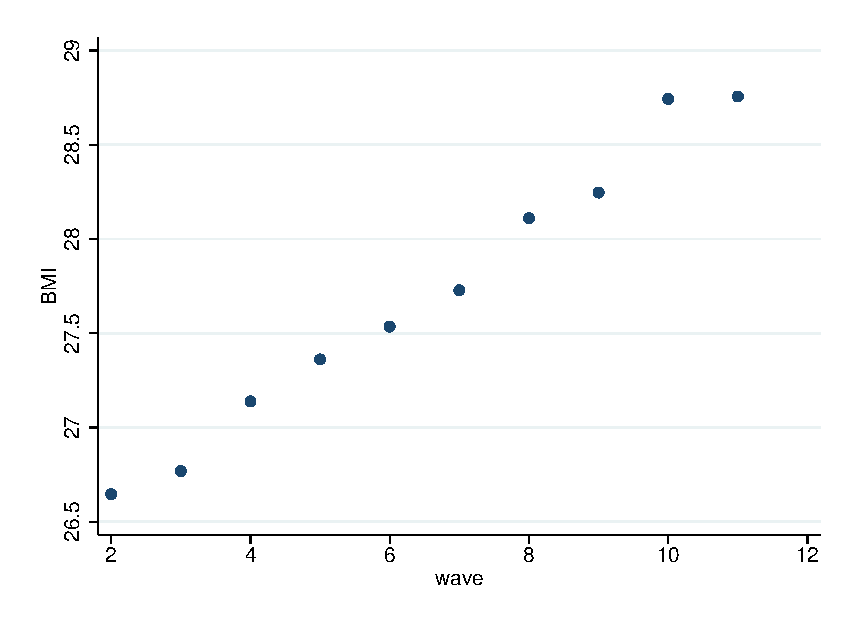
\includegraphics[width=0.6\paperwidth]{../proj/fig/wavebmi.eps}}
\caption{Mean bmi as a function of the wave}
\label{fig:wavebmi}
\end{figure}


\subsection{Tables}

\subsubsection{Descriptive Analysis}

\begin{figure}[H]
\makebox[\textwidth][c]{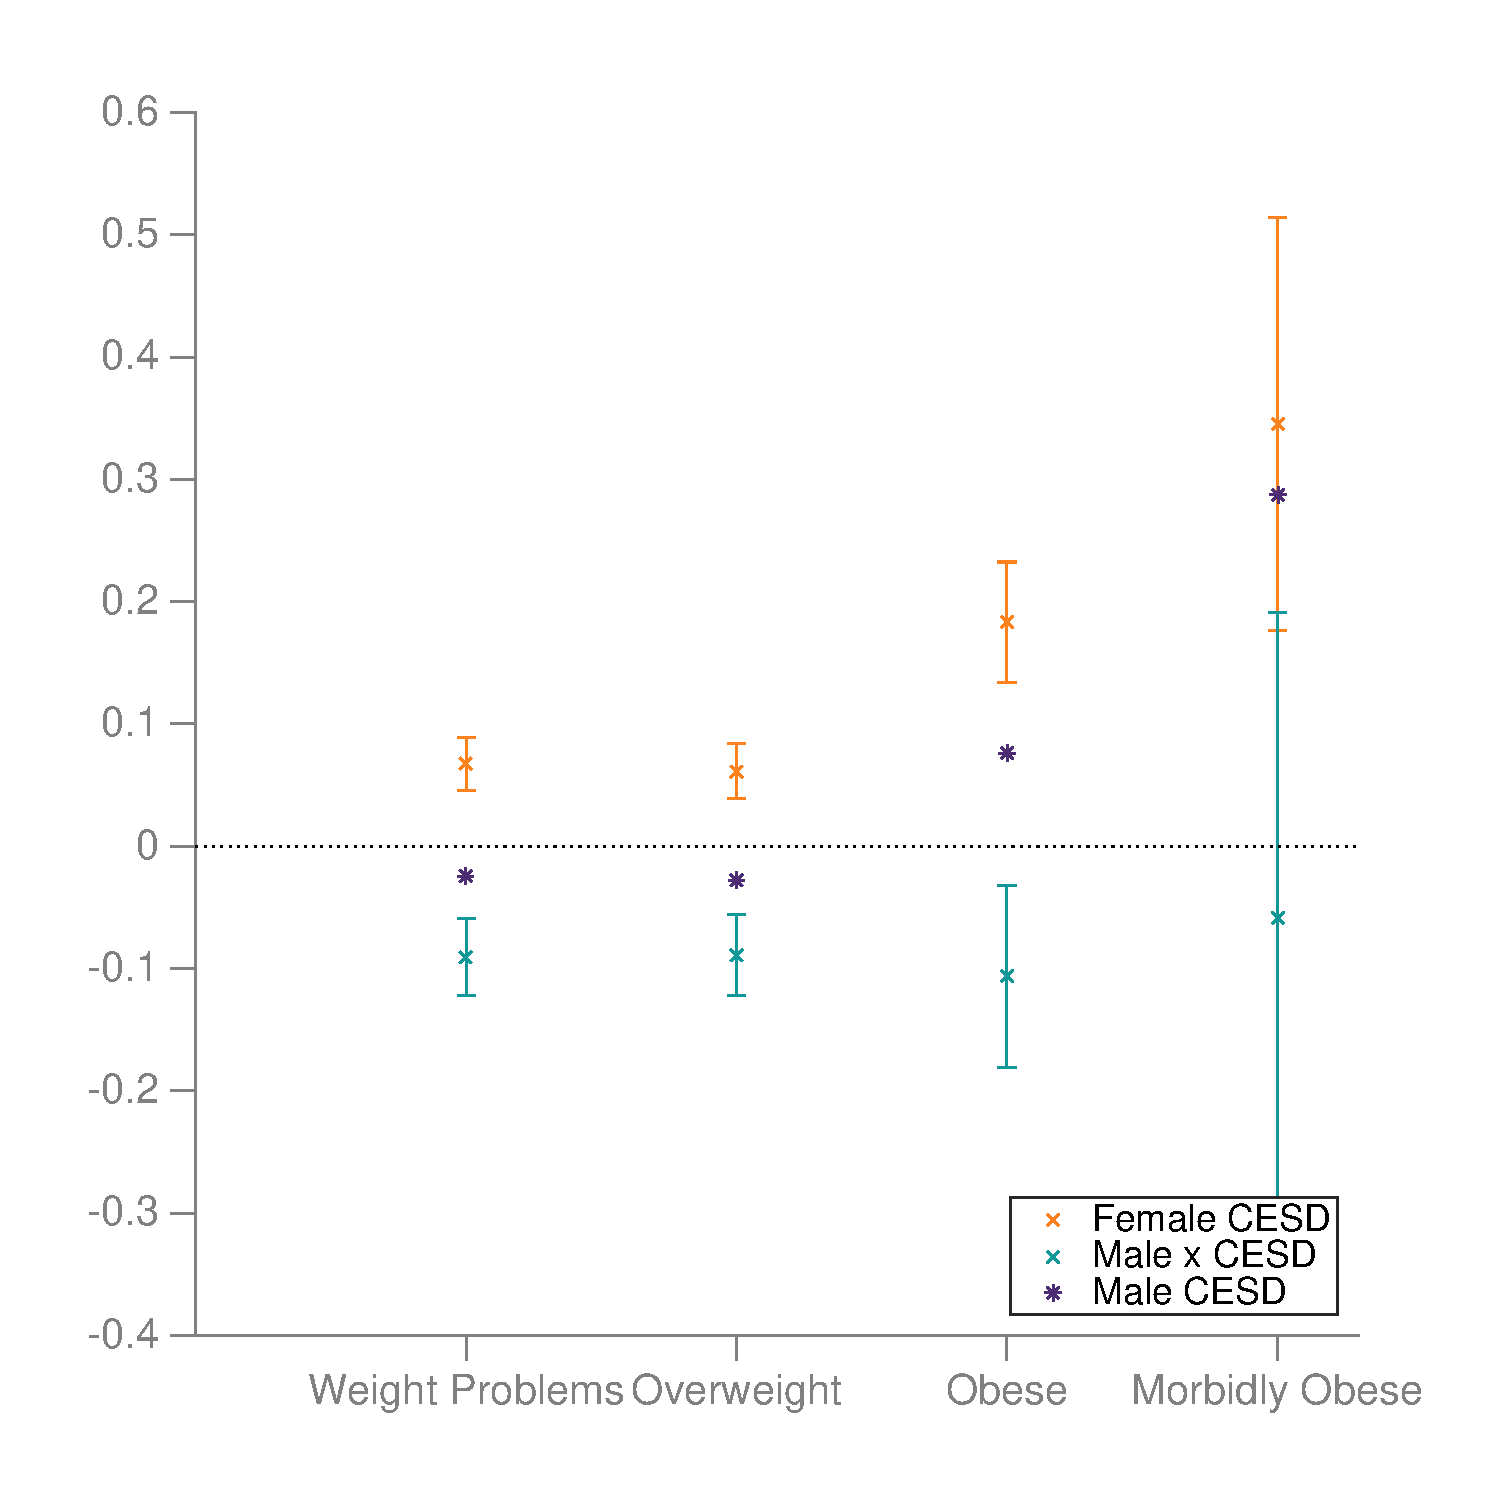
\includegraphics[width=0.6\paperwidth]{../proj/matlab/2.pdf}}
\caption{Visual representation of the obtained coefficients for CESD and both sexes, scaled by the proportion of the population in the category }
\label{fig:results2}
\end{figure}



\begin{table}[H]
\centering
{
\def\sym#1{\ifmmode^{#1}\else\(^{#1}\)\fi}
\begin{tabular}{l*{3}{c}}
\hline\hline
                    &\multicolumn{1}{c}{(1)}&\multicolumn{1}{c}{(2)}&\multicolumn{1}{c}{(3)}\\
                    &\multicolumn{1}{c}{\shortstack{weightProblems\\reg}}&\multicolumn{1}{c}{\shortstack{weightProblems\\ivreg}}&\multicolumn{1}{c}{\shortstack{weightProblems\\ivprobit marginal}}\\
\hline
CESD depression score&      0.0168\sym{***}&      0.0491\sym{***}&      0.0458\sym{***}\\
                    &   (0.00164)         &   (0.00809)         &   (0.00751)         \\
[1em]
Male x CESD         &     -0.0190\sym{***}&     -0.0665\sym{***}&     -0.0619\sym{***}\\
                    &   (0.00244)         &    (0.0110)         &    (0.0110)         \\
[1em]
Male                &       0.165\sym{***}&       0.221\sym{***}&       0.214\sym{***}\\
                    &   (0.00812)         &    (0.0149)         &    (0.0137)         \\
[1em]
has smoked          &      -0.150\sym{***}&      -0.166\sym{***}&      -0.153\sym{***}\\
                    &    (0.0120)         &    (0.0126)         &    (0.0109)         \\
[1em]
Spouse has smoked   &     0.00324         &    -0.00109         &    -0.00137         \\
                    &   (0.00782)         &   (0.00798)         &   (0.00788)         \\
[1em]
Male x has smoked   &     -0.0288         &    -0.00317         &     -0.0150         \\
                    &    (0.0159)         &    (0.0168)         &    (0.0154)         \\
[1em]
Age                 &    -0.00631\sym{***}&    -0.00620\sym{***}&    -0.00605\sym{***}\\
                    &  (0.000521)         &  (0.000523)         &  (0.000522)         \\
[1em]
Spouse's Age        &   -0.000712         &   -0.000807         &   -0.000770         \\
                    &  (0.000514)         &  (0.000516)         &  (0.000513)         \\
\hline
Observations        &      100600         &      100600         &      100600         \\
Education Control   &         Yes         &         Yes         &         Yes         \\
Wave Control        &         Yes         &         Yes         &         Yes         \\
\hline\hline
\multicolumn{4}{l}{\footnotesize \footnotesize Standard errors clustered by id in parentheses}\\
\multicolumn{4}{l}{\footnotesize \footnotesize \sym{*} \(p<0.05\), \sym{**} \(p<0.01\), \sym{***} \(p<0.001\)}\\
\end{tabular}
}

\caption{Regression results over the weight problems dependent variable}
\label{tab:weightProblems}
\end{table}

\begin{table}[H]
\centering
{
\def\sym#1{\ifmmode^{#1}\else\(^{#1}\)\fi}
\begin{tabular}{l*{3}{c}}
\hline\hline
                    &\multicolumn{1}{c}{(1)}&\multicolumn{1}{c}{(2)}&\multicolumn{1}{c}{(3)}\\
                    &\multicolumn{1}{c}{\shortstack{overweight\\reg}}&\multicolumn{1}{c}{\shortstack{overweight\\ivreg}}&\multicolumn{1}{c}{\shortstack{overweight\\ivprobit marginal}}\\
\hline
CESD depression score&      0.0152\sym{***}&      0.0445\sym{***}&      0.0412\sym{***}\\
                    &   (0.00168)         &   (0.00825)         &   (0.00769)         \\
[1em]
Male x CESD         &     -0.0190\sym{***}&     -0.0646\sym{***}&     -0.0599\sym{***}\\
                    &   (0.00249)         &    (0.0111)         &    (0.0113)         \\
[1em]
Male                &       0.176\sym{***}&       0.229\sym{***}&       0.222\sym{***}\\
                    &   (0.00823)         &    (0.0151)         &    (0.0140)         \\
[1em]
has smoked          &      -0.176\sym{***}&      -0.190\sym{***}&      -0.175\sym{***}\\
                    &    (0.0123)         &    (0.0128)         &    (0.0112)         \\
[1em]
Spouse has smoked   &     0.00248         &    -0.00135         &    -0.00174         \\
                    &   (0.00795)         &   (0.00810)         &   (0.00801)         \\
[1em]
Male x has smoked   &     -0.0123         &      0.0121         &    -0.00267         \\
                    &    (0.0162)         &    (0.0171)         &    (0.0156)         \\
[1em]
Age                 &    -0.00687\sym{***}&    -0.00677\sym{***}&    -0.00659\sym{***}\\
                    &  (0.000533)         &  (0.000535)         &  (0.000536)         \\
[1em]
Spouse's Age        &   -0.000868         &   -0.000961         &   -0.000924         \\
                    &  (0.000524)         &  (0.000525)         &  (0.000524)         \\
\hline
Observations        &      100600         &      100600         &      100600         \\
Education Control   &         Yes         &         Yes         &         Yes         \\
Wave Control        &         Yes         &         Yes         &         Yes         \\
\hline\hline
\multicolumn{4}{l}{\footnotesize \footnotesize Standard errors clustered by id in parentheses}\\
\multicolumn{4}{l}{\footnotesize \footnotesize \sym{*} \(p<0.05\), \sym{**} \(p<0.01\), \sym{***} \(p<0.001\)}\\
\end{tabular}
}

\caption{Regression results over the overweight dependent variable}
\label{tab:overweight}
\end{table}

\begin{table}[H]
\centering
{
\def\sym#1{\ifmmode^{#1}\else\(^{#1}\)\fi}
\begin{tabular}{l*{3}{c}}
\hline\hline
                    &\multicolumn{1}{c}{(1)}&\multicolumn{1}{c}{(2)}&\multicolumn{1}{c}{(3)}\\
                    &\multicolumn{1}{c}{\shortstack{obese\\reg}}&\multicolumn{1}{c}{\shortstack{obese\\ivreg}}&\multicolumn{1}{c}{\shortstack{obese\\ivprobit marginal}}\\
\hline
CESD depression score&      0.0185\sym{***}&      0.0555\sym{***}&      0.0497\sym{***}\\
                    &   (0.00168)         &   (0.00794)         &   (0.00683)         \\
[1em]
Male x CESD         &    -0.00653\sym{*}  &     -0.0317\sym{**} &     -0.0289\sym{**} \\
                    &   (0.00259)         &    (0.0111)         &    (0.0103)         \\
[1em]
Male                &      0.0336\sym{***}&      0.0688\sym{***}&      0.0636\sym{***}\\
                    &   (0.00781)         &    (0.0145)         &    (0.0137)         \\
[1em]
has smoked          &      -0.150\sym{***}&      -0.166\sym{***}&      -0.167\sym{***}\\
                    &   (0.00995)         &    (0.0106)         &    (0.0113)         \\
[1em]
Spouse has smoked   &      0.0124         &     0.00629         &     0.00580         \\
                    &   (0.00790)         &   (0.00799)         &   (0.00763)         \\
[1em]
Male x has smoked   &      0.0123         &      0.0286\sym{*}  &      0.0301         \\
                    &    (0.0134)         &    (0.0145)         &    (0.0157)         \\
[1em]
Age                 &    -0.00720\sym{***}&    -0.00706\sym{***}&    -0.00687\sym{***}\\
                    &  (0.000497)         &  (0.000498)         &  (0.000479)         \\
[1em]
Spouse's Age        &   -0.000264         &   -0.000291         &   -0.000445         \\
                    &  (0.000493)         &  (0.000495)         &  (0.000473)         \\
\hline
Observations        &      100600         &      100600         &      100600         \\
Education Control   &         Yes         &         Yes         &         Yes         \\
Wave Control        &         Yes         &         Yes         &         Yes         \\
\hline\hline
\multicolumn{4}{l}{\footnotesize \footnotesize Standard errors clustered by id in parentheses}\\
\multicolumn{4}{l}{\footnotesize \footnotesize \sym{*} \(p<0.05\), \sym{**} \(p<0.01\), \sym{***} \(p<0.001\)}\\
\end{tabular}
}

\caption{Regression results over the obese dependent variable}
\label{tab:obese}
\end{table}

\begin{table}[H]
\centering
{
\def\sym#1{\ifmmode^{#1}\else\(^{#1}\)\fi}
\begin{tabular}{l*{3}{c}}
\hline\hline
                    &\multicolumn{1}{c}{(1)}&\multicolumn{1}{c}{(2)}&\multicolumn{1}{c}{(3)}\\
                    &\multicolumn{1}{c}{\shortstack{morbidlyObese\\reg}}&\multicolumn{1}{c}{\shortstack{morbidlyObese\\ivreg}}&\multicolumn{1}{c}{\shortstack{morbidlyObese\\ivprobit marginal}}\\
\hline
CESD depression score&     0.00619\sym{***}&      0.0165\sym{***}&     0.00997\sym{***}\\
                    &  (0.000816)         &   (0.00330)         &   (0.00249)         \\
[1em]
Male x CESD         &    -0.00152         &    -0.00890\sym{*}  &    -0.00168         \\
                    &   (0.00115)         &   (0.00403)         &   (0.00367)         \\
[1em]
Male                &    -0.00887\sym{***}&     0.00132         &    -0.00948         \\
                    &   (0.00255)         &   (0.00512)         &   (0.00509)         \\
[1em]
has smoked          &     -0.0299\sym{***}&     -0.0344\sym{***}&     -0.0321\sym{***}\\
                    &   (0.00369)         &   (0.00405)         &   (0.00442)         \\
[1em]
Spouse has smoked   &     0.00843\sym{**} &     0.00671\sym{*}  &     0.00610\sym{*}  \\
                    &   (0.00314)         &   (0.00315)         &   (0.00273)         \\
[1em]
Male x has smoked   &     0.00723         &      0.0119\sym{*}  &     0.00253         \\
                    &   (0.00417)         &   (0.00470)         &   (0.00608)         \\
[1em]
Age                 &    -0.00155\sym{***}&    -0.00151\sym{***}&    -0.00152\sym{***}\\
                    &  (0.000190)         &  (0.000189)         &  (0.000166)         \\
[1em]
Spouse's Age        &   0.0000776         &   0.0000691         &  -0.0000860         \\
                    &  (0.000184)         &  (0.000183)         &  (0.000164)         \\
\hline
Observations        &      100600         &      100600         &      100600         \\
Education Control   &         Yes         &         Yes         &         Yes         \\
Wave Control        &         Yes         &         Yes         &         Yes         \\
\hline\hline
\multicolumn{4}{l}{\footnotesize \footnotesize Standard errors clustered by id in parentheses}\\
\multicolumn{4}{l}{\footnotesize \footnotesize \sym{*} \(p<0.05\), \sym{**} \(p<0.01\), \sym{***} \(p<0.001\)}\\
\end{tabular}
}

\caption{Regression results over the morbidly obese dependent variable}
\label{tab:morbidlyObese}
\end{table}

\begin{table}[H]
\centering
{
\def\sym#1{\ifmmode^{#1}\else\(^{#1}\)\fi}
\begin{tabular}{l*{3}{c}}
\hline\hline
                    &\multicolumn{1}{c}{(1)}&\multicolumn{1}{c}{(2)}&\multicolumn{1}{c}{(3)}\\
                    &\multicolumn{1}{c}{\shortstack{obese\\reg}}&\multicolumn{1}{c}{\shortstack{obese\\ivreg}}&\multicolumn{1}{c}{\shortstack{obese\\ivprobit marginal}}\\
\hline
wave==3             &      0.0219\sym{***}&      0.0232\sym{***}&      0.0251\sym{***}\\
                    &   (0.00342)         &   (0.00351)         &   (0.00394)         \\
[1em]
wave==4             &      0.0459\sym{***}&      0.0398\sym{***}&      0.0447\sym{***}\\
                    &   (0.00401)         &   (0.00437)         &   (0.00480)         \\
[1em]
wave==5             &      0.0620\sym{***}&      0.0567\sym{***}&      0.0619\sym{***}\\
                    &   (0.00438)         &   (0.00466)         &   (0.00513)         \\
[1em]
wave==6             &      0.0873\sym{***}&      0.0827\sym{***}&      0.0878\sym{***}\\
                    &   (0.00483)         &   (0.00503)         &   (0.00550)         \\
[1em]
wave==7             &      0.0959\sym{***}&      0.0915\sym{***}&      0.0962\sym{***}\\
                    &   (0.00490)         &   (0.00510)         &   (0.00553)         \\
[1em]
wave==8             &       0.126\sym{***}&       0.121\sym{***}&       0.124\sym{***}\\
                    &   (0.00525)         &   (0.00550)         &   (0.00595)         \\
[1em]
wave==9             &       0.146\sym{***}&       0.142\sym{***}&       0.145\sym{***}\\
                    &   (0.00560)         &   (0.00578)         &   (0.00618)         \\
[1em]
wave==10            &       0.161\sym{***}&       0.155\sym{***}&       0.153\sym{***}\\
                    &   (0.00539)         &   (0.00565)         &   (0.00601)         \\
[1em]
wave==11            &       0.173\sym{***}&       0.167\sym{***}&       0.165\sym{***}\\
                    &   (0.00561)         &   (0.00589)         &   (0.00625)         \\
\hline
Observations        &      100600         &      100600         &      100600         \\
Other variables ommitted&         Yes         &         Yes         &         Yes         \\
\hline\hline
\multicolumn{4}{l}{\footnotesize \footnotesize Standard errors clustered by id in parentheses}\\
\multicolumn{4}{l}{\footnotesize \footnotesize \sym{*} \(p<0.05\), \sym{**} \(p<0.01\), \sym{***} \(p<0.001\)}\\
\end{tabular}
}

\caption{Regression explaining obesity only showing the wave control}
\label{tab:wave}
\end{table}

\begin{table}[H]
\centering
{
\def\sym#1{\ifmmode^{#1}\else\(^{#1}\)\fi}
\begin{tabular}{l*{3}{c}}
\hline\hline
                    &\multicolumn{1}{c}{(1)}&\multicolumn{1}{c}{(2)}&\multicolumn{1}{c}{(3)}\\
                    &\multicolumn{1}{c}{\shortstack{obese\\reg}}&\multicolumn{1}{c}{\shortstack{obese\\ivreg}}&\multicolumn{1}{c}{\shortstack{obese\\ivprobit marginal}}\\
\hline
raeduc==2           &    0.000891         &      0.0104         &     0.00733         \\
                    &    (0.0154)         &    (0.0156)         &    (0.0141)         \\
[1em]
raeduc==3           &     -0.0196\sym{*}  &   -0.000817         &    -0.00283         \\
                    &   (0.00865)         &   (0.00973)         &   (0.00916)         \\
[1em]
raeduc==4           &     -0.0452\sym{***}&     -0.0240\sym{*}  &     -0.0267\sym{**} \\
                    &   (0.00920)         &    (0.0105)         &    (0.0100)         \\
[1em]
raeduc==5           &      -0.124\sym{***}&     -0.0974\sym{***}&      -0.101\sym{***}\\
                    &   (0.00906)         &    (0.0113)         &    (0.0116)         \\
\hline
Observations        &      100600         &      100600         &      100600         \\
Other variables ommitted&         Yes         &         Yes         &         Yes         \\
\hline\hline
\multicolumn{4}{l}{\footnotesize \footnotesize Standard errors clustered by id in parentheses}\\
\multicolumn{4}{l}{\footnotesize \footnotesize \sym{*} \(p<0.05\), \sym{**} \(p<0.01\), \sym{***} \(p<0.001\)}\\
\end{tabular}
}

\caption{Regression explaining obesity only showing the education control}
\label{tab:educ}
\end{table}

\begin{table}[H]
\centering
{
\def\sym#1{\ifmmode^{#1}\else\(^{#1}\)\fi}
\begin{tabular}{l*{2}{c}}
\hline\hline
                    &\multicolumn{1}{c}{(1)}&\multicolumn{1}{c}{(2)}\\
                    &\multicolumn{1}{c}{\shortstack{obese\\reg}}&\multicolumn{1}{c}{\shortstack{obese\\ivreg}}\\
\hline
CESD depression score&      0.0189\sym{***}&      0.0480\sym{***}\\
                    &   (0.00132)         &   (0.00578)         \\
\hline
Observations        &      100600         &      100600         \\
\hline\hline
\multicolumn{3}{l}{\footnotesize \footnotesize Standard errors clustered by id in parentheses}\\
\multicolumn{3}{l}{\footnotesize \footnotesize \sym{*} \(p<0.05\), \sym{**} \(p<0.01\), \sym{***} \(p<0.001\)}\\
\end{tabular}
}

\caption{Simplest obese regression}
\label{tab:bias}
\end{table}